
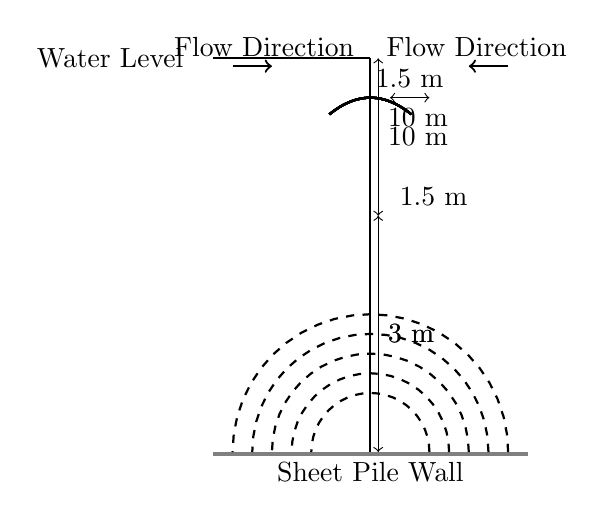
\begin{tikzpicture}[scale=0.5] % Scale the entire picture

    % Dimensions
    \def\wallHeight{6}       % Height of the sheet pile wall
    \def\waterDepth{4}        % Depth of water on the upstream side
    \def\flowWidth{8}         % Width of the flow net area

    % Draw the sheet pile wall
    \draw[thick] (0, \waterDepth) -- (0, -\wallHeight) node[below] {Sheet Pile Wall};

    % Draw impermeable bottom layer (solid rectangle)
    \fill[gray] (-\flowWidth/2, -\wallHeight) rectangle (\flowWidth/2, -\wallHeight - 0.1);
    
    % Draw water level on the left side with an arrow
    \draw[thick] (-\flowWidth/2, \waterDepth) -- (0, \waterDepth);
    
    \node[left] at (-\flowWidth/2-0.5, \waterDepth) {Water Level};

    % Add labels for physical quantities
    \node[right] at (0.2, \waterDepth-1.5) {10 m};
    \node[right] at (0.2, -\wallHeight+3) {3 m};
    \node[right] at (0.5, 0.5) {1.5 m};

    % Draw dimension indicators for wall height, water depth, and distance from wall
    \draw[<->] (0.2, \waterDepth) -- (0.2, 0) node[midway, right] {10 m};
    \draw[<->] (0.2, 0) -- (0.2, -\wallHeight) node[midway, right] {3 m};
    \draw[<->] (0.5, \waterDepth-1) -- (1.5, \waterDepth-1) node[midway, above] {1.5 m};

    % Draw flow lines (smooth curved lines around the sheet pile wall)
    \foreach \x in {-3.5, -3, -2.5, -2, -1.5, -1, 1, 1.5, 2, 2.5, 3, 3.5} {
        \draw[thick, smooth] plot[domain=-1.3:1.3] ({\x*0.8*cos(\x)}, {0.5*\wallHeight * (1 - \x*\x / 12)});
    }

    % Draw equipotential lines (semicircular lines centered at the bottom of the sheet pile wall)
    \foreach \r in {1.5, 2, 2.5, 3, 3.5} {
        \draw[thick, dashed, domain=0:180] plot ({\r*cos(\x)}, {-\wallHeight + \r*sin(\x)});
    }

    % Draw arrows to show flow direction
    \draw[->, thick] (-\flowWidth/2+0.5, \waterDepth-0.2) -- (-\flowWidth/2+1.5, \waterDepth-0.2);
    \draw[->, thick] (\flowWidth/2-0.5, \waterDepth-0.2) -- (\flowWidth/2-1.5, \waterDepth-0.2);
    
    % Label for the flow direction
    \node at (-\flowWidth/2+1.3, \waterDepth+0.3) {Flow Direction};
    \node at (\flowWidth/2-1.3, \waterDepth+0.3) {Flow Direction};

\end{tikzpicture}

